\begin{lstlisting}
•    Section 4.5:  3,  5,  8,  11  
•    Section 4.6:  7,  8,  9,  10
\end{lstlisting}
\begin{exercise}
\begin{figure}[H]
\centering
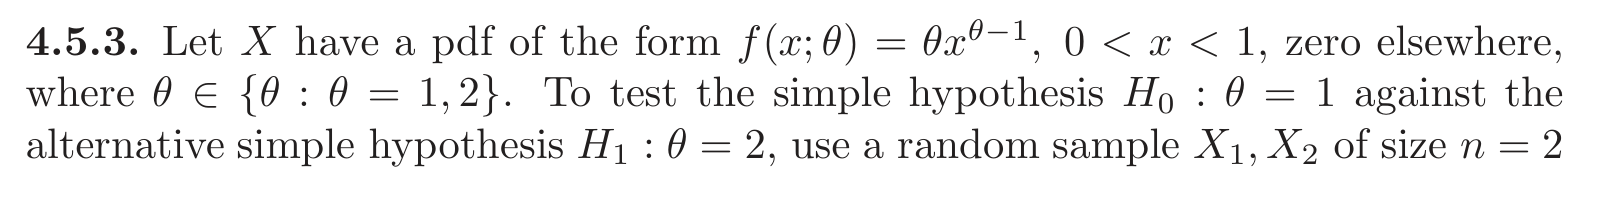
\includegraphics[width=\textwidth]{hw6-2025041423.png}
% \caption{}
\label{}
\end{figure}
\begin{figure}[H]
\centering

\includegraphics[width=\textwidth]{1-hw6-2025041423.png}
% \caption{}
\label{}
\end{figure}
\end{exercise}
The power function is
\[
\begin{aligned}
\beta(\theta) & =\mathbb{P}_{\theta}((X_1,X_2)\in C)=\mathbb{P}_{\theta}\left( X_1X_2\geq \frac{3}{4} \right) \\
 & =\int_{0}^{1} \int_{0}^{1} \mathbb{1}_{\left\{  x_1x_2\geq \frac{3}{4}  \right\}} \cdot \underbrace{ f(x_1;\theta)f(x_2;\theta) }_{ =\theta^{2}\cdot x_1^{\theta-1}x_2^{\theta-1} } \, \mathrm{d}x_1  \, \mathrm{d}x_2  \\
 & =\int_{\frac{3}{4}}^{1} \int_{\frac{3}{4x_1} }^{1} \theta^{2}\cdot x_1^{\theta-1}x_2^{\theta-1} \, \mathrm{d}x_2  \, \mathrm{d}x_1 \\
  & =\int_{\frac{3}{4}}^{1} \theta \cdot\left( 1-\left( \frac{3}{4x_1} \right)^{\theta} \right) \, \mathrm{d}x_1 \\
  & =\int_{\frac{3}{4}}^{1} \theta-\left( \frac{3}{4} \right)^{\theta}x_1^{-\theta} \, \mathrm{d}x_1  \\
 & =\begin{cases}
\frac{1}{4}+\frac{3}{4}\ln\frac{3}{4}  & \theta=1 \\
\frac{5}{16} & \theta=2  
\end{cases}
\end{aligned}
\]
\begin{exercise}
\begin{figure}[H]
\centering
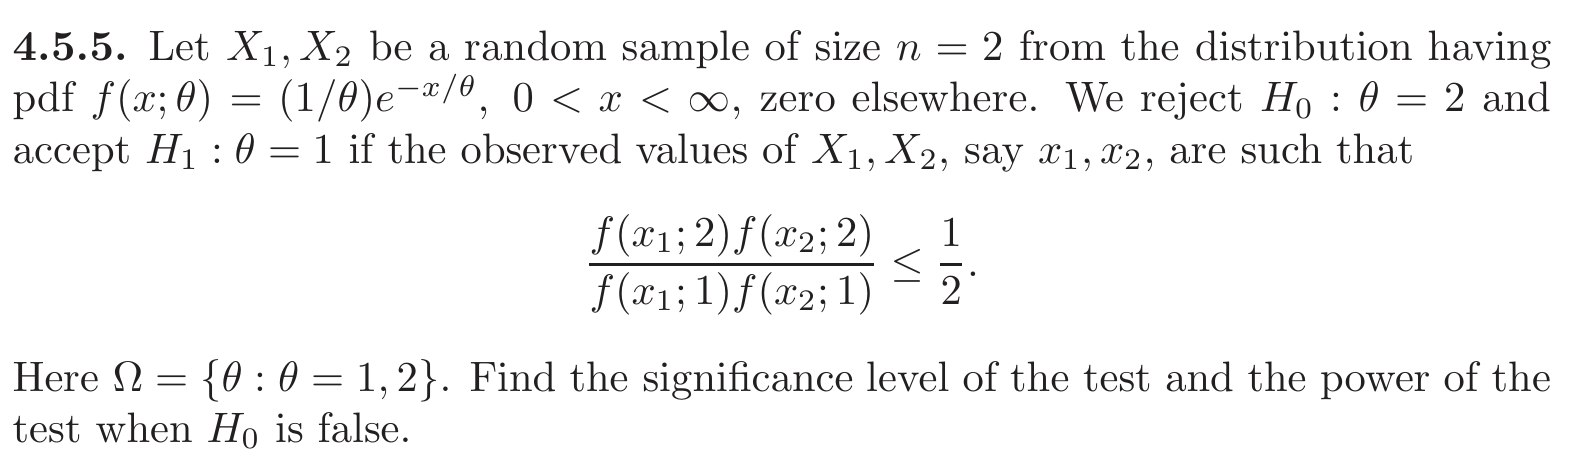
\includegraphics[width=\textwidth]{2-hw6-2025041423.png}
% \caption{}
\label{}
\end{figure}
\end{exercise}
The rejection set $R$ is
\[
\begin{aligned}
\left\{  (x_1,x_2):\frac{f(x_1;2)f(x_2;2)}{f(x_1;1)f(x_2;1)}\leq \frac{1}{2}  \right\} & =\left\{  (x_1,x_2):\frac{\frac{1}{2}e^{ -x_1/2 }\cdot\frac{1}{2}e^{ -x_2/2 }}{e^{ -x_1 }\cdot e^{ -x_2 }}\leq \frac{1}{2}  \right\} \\
 & =\{ (x_1,x_2):e^{ (x_1+x_2)/2 }\leq 2 \} \\
 & =\{ (x_1,x_2):x_1+x_2\leq 2\ln2 \}
\end{aligned}
\]
The power of the test is
\[
\begin{aligned}
\beta(\theta) & =\mathbb{P}_{\theta}((X_1,X_2)\in R) \\
 & =\int_{0}^{\infty} \int_{0}^{\infty} \mathbb{1}_{\{ x_1+x_2\leq 2\ln2 \}}\cdot \theta ^{-1}e^{ -x_1/\theta }\cdot\theta ^{-1}e^{ -x_2/\theta } \, \mathrm{d}x_2 \, \mathrm{d}x_1 \\
 & =\int_{0}^{2\ln2} \int_{0}^{2\ln2-x_1}  \theta ^{-1}e^{ -x_1/\theta }\cdot\theta ^{-1}e^{ -x_2/\theta } \, \mathrm{d}x_2  \, \mathrm{d}x_1 \\
 & =1-\frac{4^{-1/\theta } (\theta +2\ln 2)}{\theta } 
\end{aligned} 
\]
The significance level of the test is
\[
\alpha=\sup_{\theta\in\Theta_0=\{ 2 \}}\beta(\theta)=\beta(2)=1-\frac{4^{-\frac{1}{2}}(2+2\ln2)}{2}=\frac{1}{2}-\frac{1}{2}\ln2
\]
When $H_0$ is false, $\theta=1$, then
\[
\beta(1)=1-\frac{4^{-1}(1+2\ln2)}{1}=\frac{3}{4}-\frac{1}{2}\ln2
\]
\begin{exercise}
\begin{figure}[H]
\centering
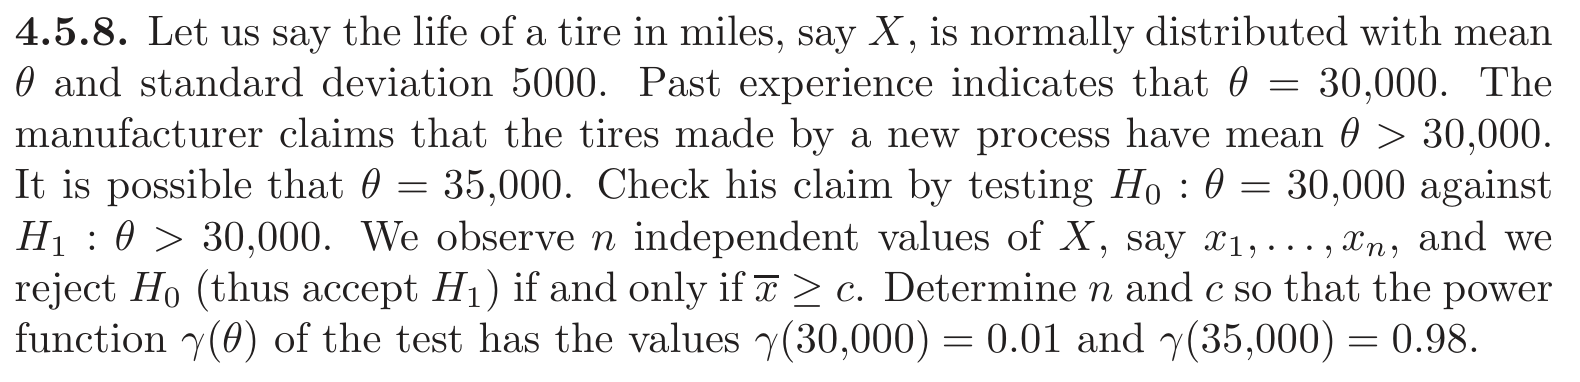
\includegraphics[width=\textwidth]{3-hw6-2025041423.png}
% \caption{}
\label{}
\end{figure}
\end{exercise}
\[
X\sim N(\theta,\sigma^{2})=N(30000,5000^2)
\]
\[
\overline{X}_n=\frac{\sum_{k=1}^{n} X_k}{n}\sim N(\theta,\sigma^{2}/n)
\]
\[
\sqrt{ n }\cdot\frac{\overline{X}_n-\theta}{\sigma}\sim N(0,1)
\]
\[
\overline{X}_n\geq c\iff \sqrt{ n }\cdot\frac{\overline{X}_n-\theta}{\sigma}\geq \sqrt{ n }\cdot\frac{c-\theta}{\sigma}
\]
The power function is
\[
\gamma(\theta)=\mathbb{P}_{\theta}((X_1,\dots,X_n)\in R)=\mathbb{P}_{\theta}\left( \sqrt{ n }\cdot\frac{\overline{X}_n-\theta}{\sigma}\geq \sqrt{ n }\cdot\frac{c-\theta}{\sigma} \right)=1-\Phi\left( \sqrt{ n }\cdot\frac{c-\theta}{\sigma} \right)
\]
Let $\gamma(30000)=0.01$ and $\gamma(35000)=0.98$ then
\[
\begin{aligned}
\sqrt{ n }\cdot\frac{c-30000}{5000} & =\Phi ^{-1}(0.99)\approx 2.326\\
\sqrt{ n }\cdot\frac{c-35000}{5000} & =\Phi ^{-1}(0.02)\approx-2.054
\end{aligned}
\]
We have
\[
n\approx19.1844,\qquad c \approx32655.3
\]
\begin{exercise}
\begin{figure}[H]
\centering
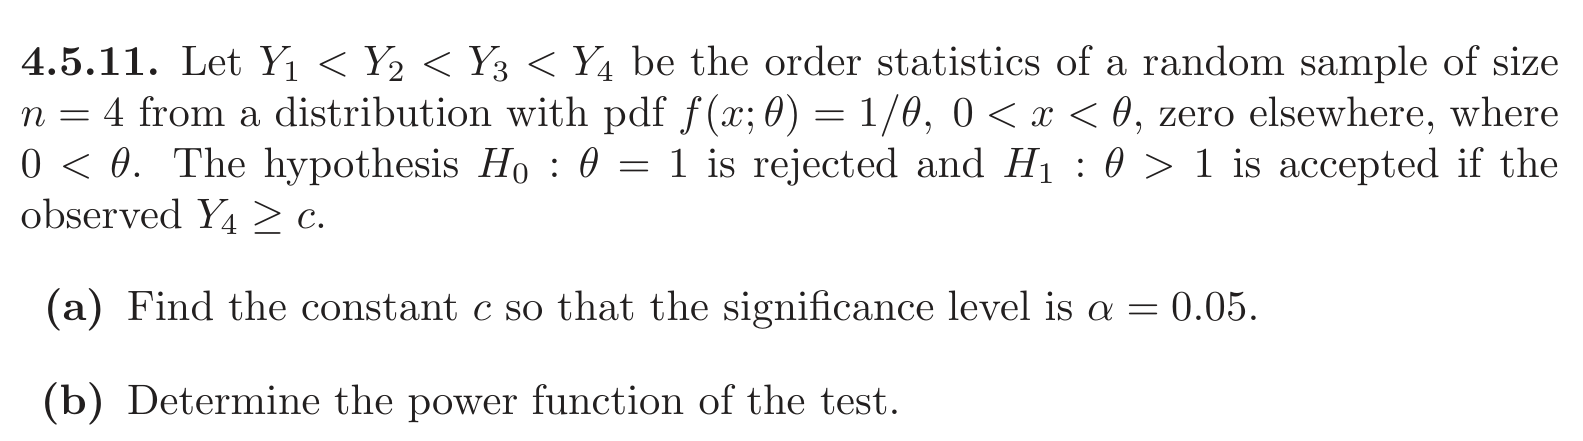
\includegraphics[width=\textwidth]{4-hw6-2025041423.png}
% \caption{}
\label{}
\end{figure}
\end{exercise}
(1) Clearly, $c\in(0,\theta)$, then
\[
\begin{aligned}
\beta(\theta) & =\mathbb{P}_{\theta}(Y_4\geq c)=1-\mathbb{P}_{\theta}(Y_4<c)=1-\mathbb{P}_{\theta}(X_i<c;i=1,2,3,4) \\
 & =1-\left( \int_{0}^{c}  \frac{1}{\theta } \, \mathrm{d}x  \right)^{4}=1-\frac{c^{4}}{\theta^{4}}
\end{aligned}
\]
\[
\alpha=\sup_{\theta\in\Theta_0=\{ 1 \}}\beta(\theta)=1-c^{4}
\]
Let $\alpha=0.05$ then $c=\left( \frac{19}{20} \right)^{\frac{1}{4}}$.

(2) the power function is
\[
\beta(\theta)=\begin{cases}
1 & c\leq 0 \\
1-\frac{c^{4}}{\theta^{4}} & 0<c<\theta \\
0 & c\geq \theta
\end{cases}
\]
\begin{exercise}
\begin{figure}[H]
\centering
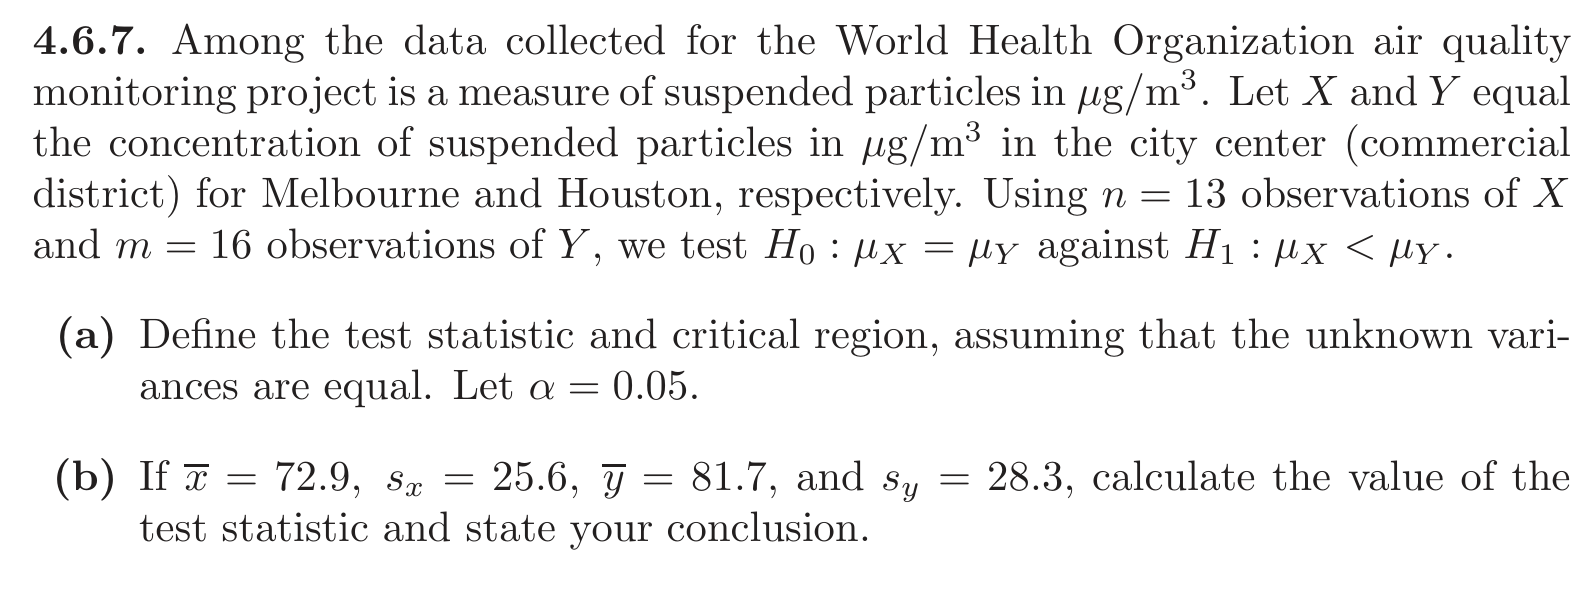
\includegraphics[width=\textwidth]{5-hw6-2025041423.png}
% \caption{}
\label{}
\end{figure}
\end{exercise}
(a) Let's test the null hypothesis that $\mu_{X}=\mu_{Y}$. Write this as $H_0:\delta=0$, $H_1:\delta>0$ where $\delta=\mu_{Y}-\mu_{X}$. The nonparametric plug-in estimate of $\delta$ is  $\widehat{\delta}=\overline{Y}-\overline{X}$, with estimated standard error
\[
\widehat{\text{se}}=\sqrt{ \frac{s_x^2}{n}+\frac{s_{y}^2}{m} }
\]
By Student's theorem, the random variable
\[
T\coloneqq \frac{(\overline{Y}-\overline{X})-(\mu_{Y}-\mu_{X})}{\left( \frac{1}{n+m-1}\left[ (n-1)S_{X}^2+(m-1)S_{Y}^2 \right] \right)^{\frac{1}{2}}/\sqrt{ n+m }}\sim t(n+m-1)
\]
\[
\alpha=\mathbb{P}_{H_0}(\widehat{\delta}>c)=\mathbb{P}_{H_0}\left( T>\frac{c\sqrt{ n+m }}{\sqrt{ \frac{1}{n+m-1}[(n-1)S_{X}^2+(m-1)S_{Y}^2] }} \right)
\]
Let
\[
c=\frac{\sqrt{ (n+m)(n+m-1) }}{\sqrt{ (n-1)S_{X}^2+(m-1)S_{Y}^2 }}t_{n+m-1,0.05}=\frac{28.4956}{\sqrt{ 12S_{X}^2+15S_{Y}^2 }}\cdot1.701=\frac{48.471}{\sqrt{ 12S_{X}^2+15S_{Y}^2 }}
\]
The critical region of $\widehat{\delta}$ is
\[
(\frac{48.471}{\sqrt{ 12S_{X}^2+15S_{Y}^2 }},+\infty)
\]
(b) Let $\overline{x}=72.9,s_{x}=25.6,\overline{y}=81.7,s_{y}=28.3,n=13,m=16$, then
\[
p\text{ -value}=\mathbb{P}\left( T>\frac{\overline{y}-\overline{x}}{\left( \frac{1}{n+m-1}[(n-1)s_{x}^2+(m-1)s_{y}^2] \right)^{\frac{1}{2}}/\sqrt{ n+m }} \right)=\mathbb{P}(T>0.86859)
\]
$0.86859<1.703$,因此在 $95\%$ 显著性水平下有理由拒绝零假设,即休斯顿市中心悬浮颗粒密度大于墨尔本.

\begin{exercise}
\begin{figure}[H]
\centering
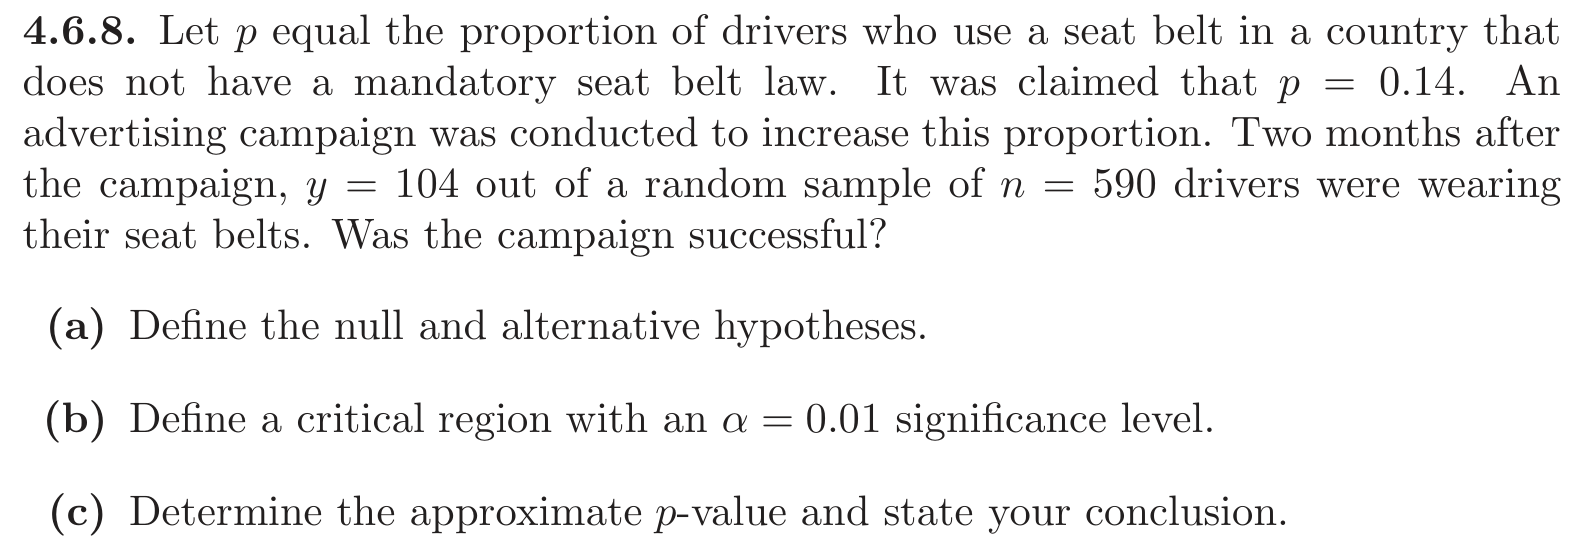
\includegraphics[width=\textwidth]{6-hw6-2025041423.png}
% \caption{}
\label{}
\end{figure}
\end{exercise}
(a) $H_0:p=0.14,H_1:p>0.14$.

(b) $p_0=0.14$, let $X_1,\dots,X_n$ be random sample of $X\sim b(1,p)$, $n=590$. Then the estimator of $p$ is $\widehat{p}=\overline{X}$. Define
\[
Z=\frac{\widehat{p}-p_0}{\sqrt{ p_0(1-p_0)/n }}
\]
Then $Z\sim N(0,1)$, and
\[
\alpha=\mathbb{P}_{H_0}(\widehat{p}\in C)
\]
\[
C=(p_0+\sqrt{ p_0(1-p_0)/n }\cdot z_{\alpha},+\infty)=(0.173227,+\infty )
\]
(c) $\widetilde{p}=\frac{y}{n}=\frac{104}{590}$ then
\[
p\text{ -value}=\mathbb{P}\left( Z\geq \frac{\widetilde{p}-p_0}{\sqrt{ p_0(1-p_0)/n }} \right)=\mathbb{P}(Z\geq 2.53907)=0.00555739<\alpha
\]
所以认为广告战役成功.

\begin{lstlisting}[language=mathematica]
dist = NormalDistribution[0, 1]
CDF[dist, 2.53907]
1 - %
\end{lstlisting}
\begin{exercise}
\begin{figure}[H]
\centering
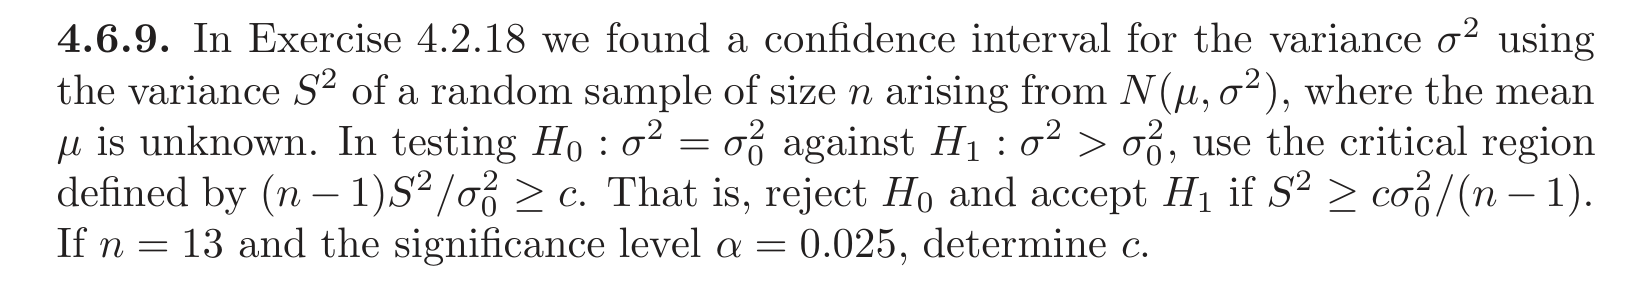
\includegraphics[width=\textwidth]{7-hw6-2025041423.png}
% \caption{}
\label{}
\end{figure}
\begin{figure}[H]
\centering
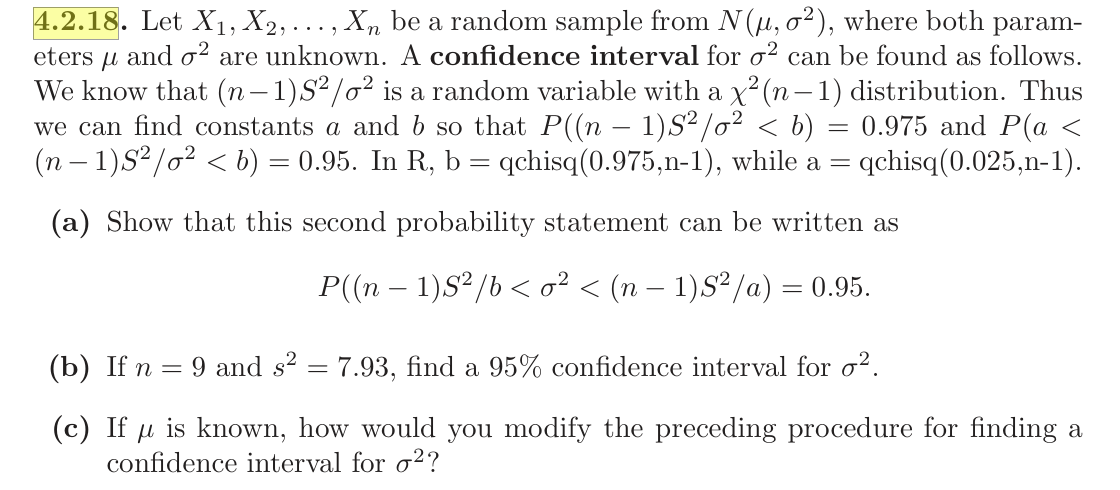
\includegraphics[width=\textwidth]{hw6-2025041515.png}
% \caption{}
\label{}
\end{figure}
\end{exercise}
\[
W\coloneqq (n-1)S^2/\sigma^{2}\sim \chi^{2}(n-1)
\]
\[
\alpha=\mathbb{P}_{H_0}((X_1,\dots,X_n)\in \{ S^2\geq c\sigma_0^2/(n-1) \})=\mathbb{P}(W\geq c)
\]
Then $c=\chi^{2}_{n-1,\alpha}=\chi^{2}_{12,0.025}=23.337$.

\begin{exercise}
\begin{figure}[H]
\centering
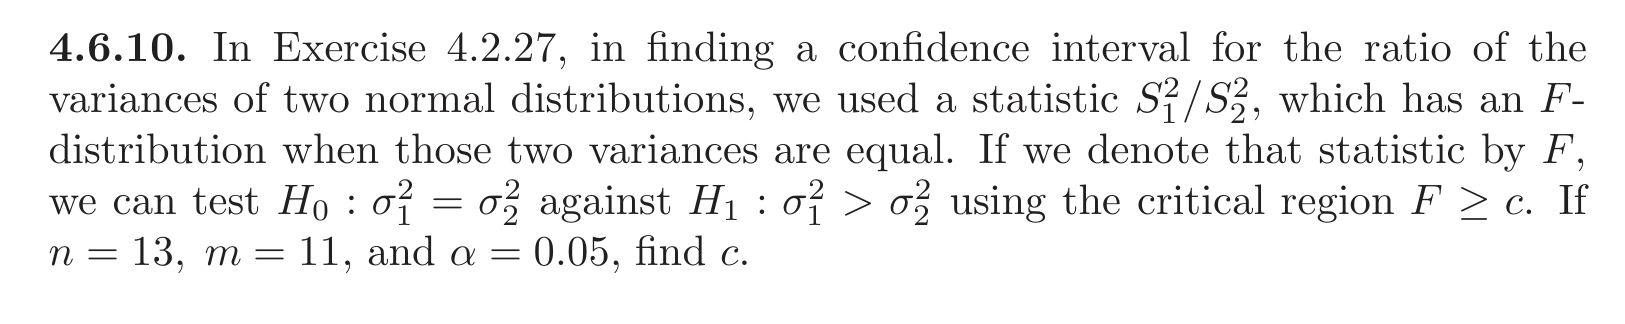
\includegraphics[width=\textwidth]{8-hw6-2025041423.png}
% \caption{}
\label{}
\end{figure}
\begin{figure}[H]
\centering
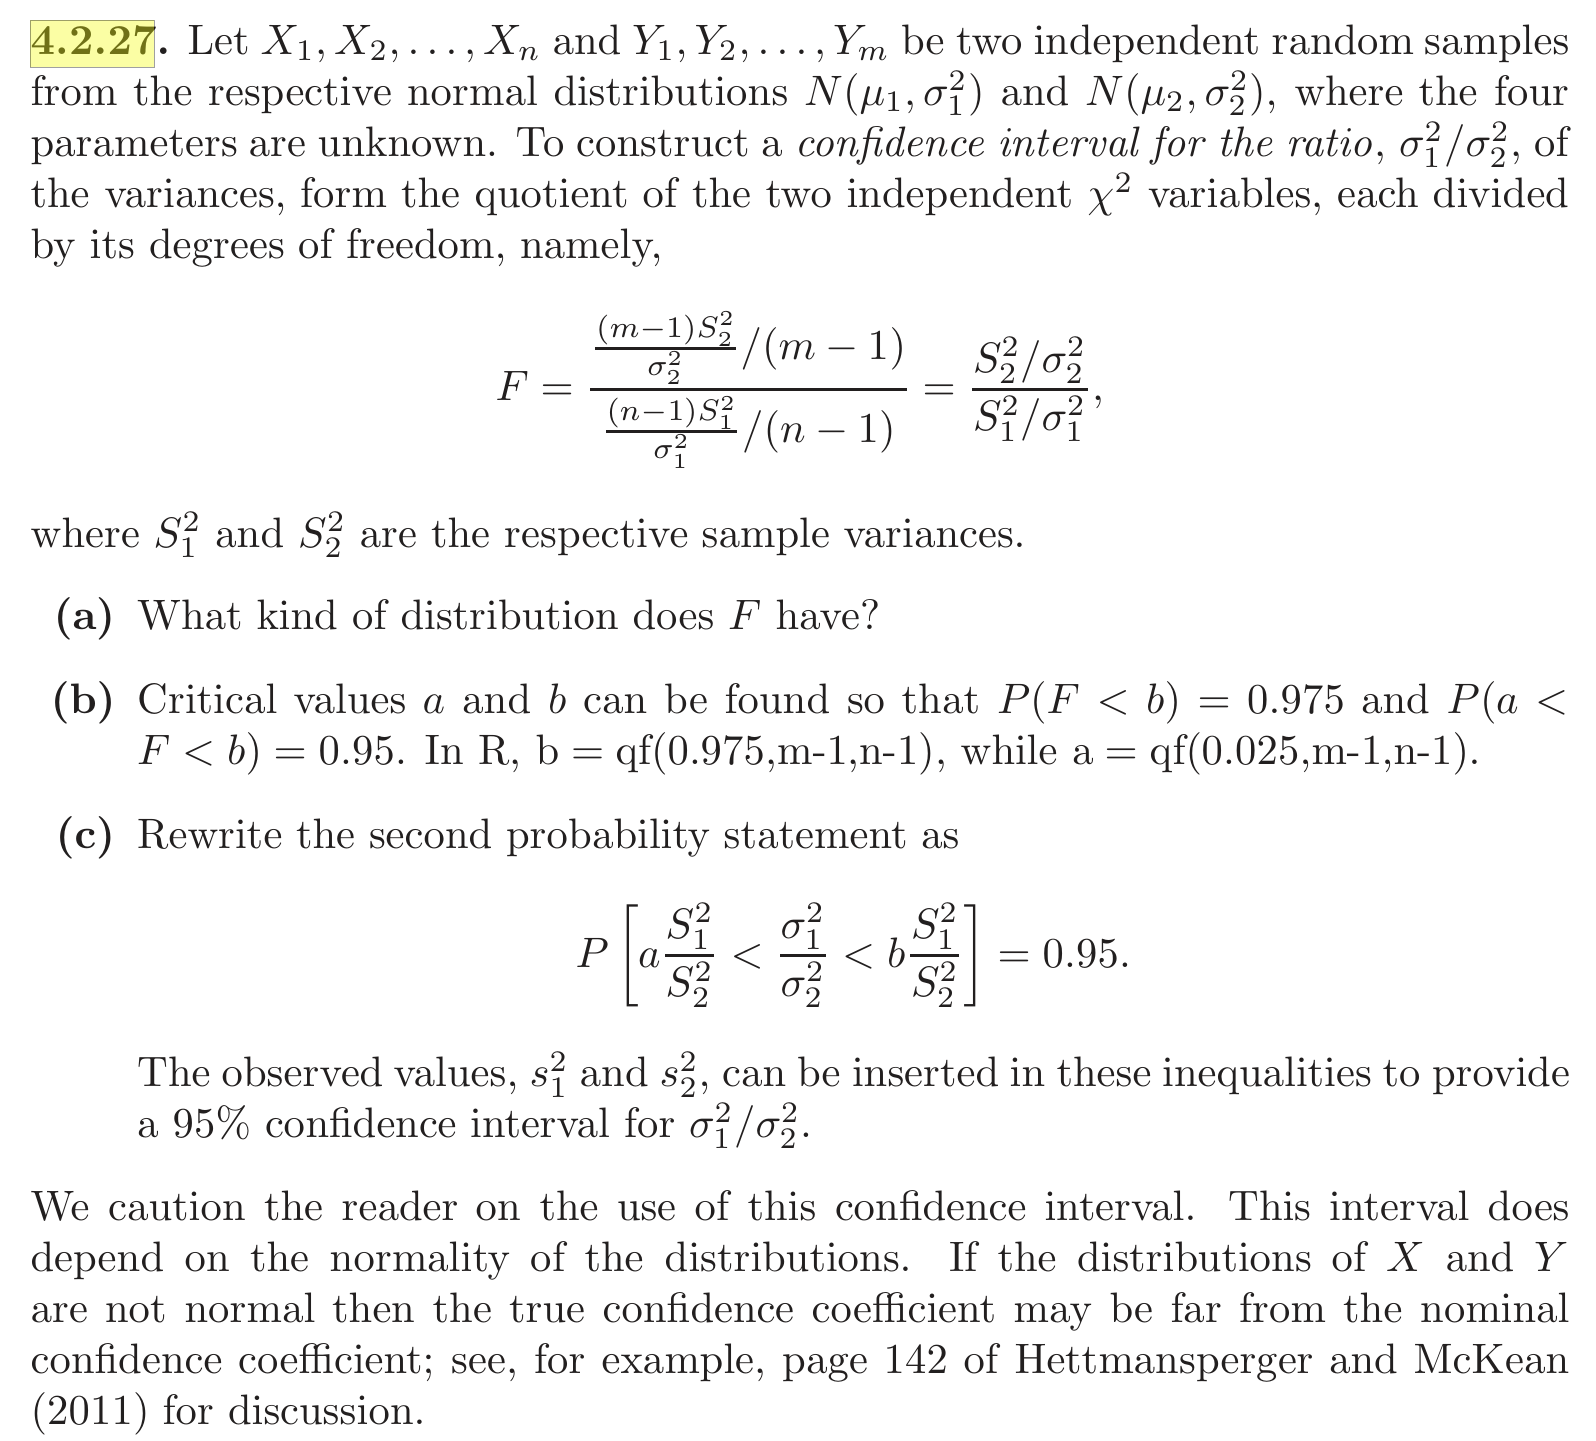
\includegraphics[width=\textwidth]{9-hw6-2025041423.png}
% \caption{}
\label{}
\end{figure}
\end{exercise}
When $\sigma^{2}_{1}=\sigma_2^2$,
\[
F=\frac{S_1^2}{S_2^2}=\frac{\frac{(n-1)S_1^2}{\sigma_1^2}/(n-1)}{\frac{(m-1)S_2^2}{\sigma_2^2}/(m-1)}\sim F(n-1,m-1)
\]
\[
\alpha=\mathbb{P}_{H_0}(F>c)
\]
\[
c=F_{\alpha}(n,m)=F_{0.05}(12,10)=2.91298
\]
\begin{lstlisting}[language=mathematica]
fDist = FRatioDistribution[12, 10]
Quantile[fDist, 0.95]
\end{lstlisting}